\section{EMPIRICAL EVALUATION} \label{sec:exp}


\begin{table*}[t]
\centering
\caption{Comparison of pruning algorithms for size constraint experiments (best combined metric in bold); *Values as reported in  \cite{ireland2022lense} and ``--" denotes no reasonable result is achieved by the corresponding algorithm under the time constraint.}
\vspace{1em}
\label{tab:size_constraint}
\resizebox{\textwidth}{!}{%
\begin{tabular}{|ccccccccccccccccccc|}
\hline
\multicolumn{1}{|c|}{}         & \multicolumn{3}{c|}{\qs}                                               & \multicolumn{3}{c|}{SS}                                               & \multicolumn{3}{c|}{\gcomb*}                                         & \multicolumn{3}{c|}{\comb}                                            & \multicolumn{3}{c|}{\lense*}                                          & \multicolumn{3}{c|}{\gnn}                        \\ \hline
\multicolumn{1}{|c|}{Graph}    & $P_r \uparrow$  & $P_g$ $\uparrow$ & \multicolumn{1}{c|}{$C \uparrow$} & $P_r \uparrow$  & $P_g$ $\uparrow$ & \multicolumn{1}{c|}{$C\uparrow$} & $P_r \uparrow$ & $P_g$ $\uparrow$ & \multicolumn{1}{c|}{$C\uparrow$} & $P_r \uparrow$  & $P_g$ $\uparrow$ & \multicolumn{1}{c|}{$C\uparrow$} & $P_r \uparrow$ & $P_g$ $\uparrow$ & \multicolumn{1}{c|}{$C\uparrow$} & $P_r \uparrow$  & $P_g$ $\uparrow$ & $C\uparrow$ \\ \hline
& \multicolumn{18}{c|}{\textbf{Maximum Cover}}  \\ \hline
\multicolumn{1}{|c||}{Facebook}& 1.0000& 0.9953& \multicolumn{1}{c||}
{\textbf{0.9953}}& 0.9884& 0.9027& \multicolumn{1}{c||}
{0.8922}& 0.9270& 0.0700& \multicolumn{1}{c||}
{0.0649}& 1.0000& 0.3840& \multicolumn{1}{c||}
{0.3840}& 0.9660& 0.0700& \multicolumn{1}{c||}
{0.0676}& 1.0000& 0.7697& \multicolumn{1}{c|}
{0.7697}\\
\multicolumn{1}{|c||}{Wiki}& 0.9998& 0.9422& \multicolumn{1}{c||}
{\textbf{0.9420}}& 0.9559& 0.9346& \multicolumn{1}{c||}
{0.8934}& 0.9900& 0.0300& \multicolumn{1}{c||}
{0.0297}& 1.0000& 0.4528& \multicolumn{1}{c||}
{0.4528}& 1.0940& 0.3400& \multicolumn{1}{c||}
{0.3720}& 1.0000& 0.9199& \multicolumn{1}{c|}
{0.9199}\\
\multicolumn{1}{|c||}{Deezer}& 0.9606& 0.9797& \multicolumn{1}{c||}
{0.9411}& 0.9870& 0.9855& \multicolumn{1}{c||}
{\textbf{0.9727}}& 0.9940& 0.1300& \multicolumn{1}{c||}
{0.1292}& 1.0000& 0.7278& \multicolumn{1}{c||}
{0.7278}& 0.9790& 0.7500& \multicolumn{1}{c||}
{0.7343}& 1.0000& 0.9151& \multicolumn{1}{c|}
{0.9151}\\
\multicolumn{1}{|c||}{Slashdot}& 1.0000& 0.9925& \multicolumn{1}{c||}
{\textbf{0.9925}}& 0.9824& 0.9889& \multicolumn{1}{c||}
{0.9715}& 1.0000& 0.0200& \multicolumn{1}{c||}
{0.0200}& 1.0000& 0.9844& \multicolumn{1}{c||}
{0.9844}& 0.9790& 0.6900& \multicolumn{1}{c||}
{0.6755}& 1.0000& 0.9810& \multicolumn{1}{c|}
{0.9810}\\
\multicolumn{1}{|c||}{Twitter}& 0.9929& 0.9911& \multicolumn{1}{c||}
{\textbf{0.9841}}& 0.9306& 0.9893& \multicolumn{1}{c||}
{0.9206}& 0.9970& 0.1700& \multicolumn{1}{c||}
{0.1695}& 1.0000& 0.5654& \multicolumn{1}{c||}
{0.5654}& 0.9890& 0.3300& \multicolumn{1}{c||}
{0.3264}& 0.9987& 0.9793& \multicolumn{1}{c|}
{0.9780}\\
\multicolumn{1}{|c||}{DBLP}& 0.9951& 0.9957& \multicolumn{1}{c||}
{\textbf{0.9908}}& 0.9945& 0.9963& \multicolumn{1}{c||}
{\textbf{0.9908}}& 0.9990& 0.0300& \multicolumn{1}{c||}
{0.0300}& 1.0000& 0.1818& \multicolumn{1}{c||}
{0.1818}& 0.9900& 0.9000& \multicolumn{1}{c||}
{0.8910}& 1.0000& 0.8705& \multicolumn{1}{c|}
{0.8705}\\
\multicolumn{1}{|c||}{YouTube}& 1.0000& 0.9995& \multicolumn{1}{c||}
{\textbf{0.9995}}& 0.9999& 0.9987& \multicolumn{1}{c||}
{0.9986}& 0.9980& 0.0700& \multicolumn{1}{c||}
{0.0699}& 1.0000& 0.9572& \multicolumn{1}{c||}
{0.9572}& 0.9820& 0.7900& \multicolumn{1}{c||}
{0.7758}& 0.9947& 0.9967& \multicolumn{1}{c|}
{0.9914}\\
\multicolumn{1}{|c||}{Skitter}& 0.9985& 0.9997& \multicolumn{1}{c||}
{0.9982}& 0.9857& 0.9991& \multicolumn{1}{c||}
{0.9848}& 0.9990& 0.1000& \multicolumn{1}{c||}
{0.0999}& --& --& \multicolumn{1}{c||}
{--}& 0.9760& 0.7000& \multicolumn{1}{c||}
{0.6832}& 0.9993& 0.9891& \multicolumn{1}{c|}
{\textbf{0.9884}}\\
\hline
& \multicolumn{18}{c|}{\textbf{Maximum Cut}}  \\ \hline
\multicolumn{1}{|c||}{Facebook}& 0.9886& 0.7935& \multicolumn{1}{c||}
{0.7845}& 0.9928& 0.9027& \multicolumn{1}{c||}
{\textbf{0.8962}}& 0.8130& 0.9500& \multicolumn{1}{c||}
{0.7723}& 1.0000& 0.1538& \multicolumn{1}{c||}
{0.1538}& 1.0000& 0.0700& \multicolumn{1}{c||}
{0.0700}& 1.0000& 0.6774& \multicolumn{1}{c|}
{0.6774}\\
\multicolumn{1}{|c||}{Wiki}& 0.9985& 0.9037& \multicolumn{1}{c||}
{0.9023}& 0.9981& 0.9346& \multicolumn{1}{c||}
{\textbf{0.9328}}& 0.9200& 0.9600& \multicolumn{1}{c||}
{0.8832}& 1.0000& 0.7011& \multicolumn{1}{c||}
{0.7011}& 0.9810& 0.3900& \multicolumn{1}{c||}
{0.3826}& 1.0000& 0.9004& \multicolumn{1}{c|}
{0.9004}\\
\multicolumn{1}{|c||}{Deezer}& 0.9996& 0.9730& \multicolumn{1}{c||}
{0.9726}& 0.9999& 0.9855& \multicolumn{1}{c||}
{\textbf{0.9854}}& 0.8500& 0.9900& \multicolumn{1}{c||}
{0.8415}& 1.0000& 0.3754& \multicolumn{1}{c||}
{0.3754}& 0.9750& 0.7400& \multicolumn{1}{c||}
{0.7215}& 1.0000& 0.9188& \multicolumn{1}{c|}
{0.9188}\\
\multicolumn{1}{|c||}{Slashdot}& 1.0000& 0.9904& \multicolumn{1}{c||}
{\textbf{0.9904}}& 1.0000& 0.9889& \multicolumn{1}{c||}
{0.9889}& 0.6320& 0.9900& \multicolumn{1}{c||}
{0.6257}& 0.7935& 0.9929& \multicolumn{1}{c||}
{0.7879}& 0.9900& 0.6200& \multicolumn{1}{c||}
{0.6138}& 1.0000& 0.9797& \multicolumn{1}{c|}
{0.9797}\\
\multicolumn{1}{|c||}{Twitter}& 1.0000& 0.9900& \multicolumn{1}{c||}
{\textbf{0.9900}}& 1.0000& 0.9893& \multicolumn{1}{c||}
{0.9893}& 0.6280& 0.9900& \multicolumn{1}{c||}
{0.6217}& 1.0000& 0.5542& \multicolumn{1}{c||}
{0.5542}& 0.9870& 0.4800& \multicolumn{1}{c||}
{0.4738}& 1.0000& 0.9740& \multicolumn{1}{c|}
{0.9740}\\
\multicolumn{1}{|c||}{DBLP}& 1.0000& 0.9954& \multicolumn{1}{c||}
{0.9954}& 1.0000& 0.9963& \multicolumn{1}{c||}
{\textbf{0.9963}}& 0.6460& 0.9900& \multicolumn{1}{c||}
{0.6395}& 1.0000& 0.1825& \multicolumn{1}{c||}
{0.1825}& 0.9930& 0.9200& \multicolumn{1}{c||}
{0.9136}& 1.0000& 0.8623& \multicolumn{1}{c|}
{0.8623}\\
\multicolumn{1}{|c||}{YouTube}& 1.0000& 0.9994& \multicolumn{1}{c||}
{\textbf{0.9994}}& 1.0000& 0.9987& \multicolumn{1}{c||}
{0.9987}& 0.5360& 0.9900& \multicolumn{1}{c||}
{0.5306}& 0.9990& 0.9705& \multicolumn{1}{c||}
{0.9695}& 0.9870& 0.7900& \multicolumn{1}{c||}
{0.7797}& 0.9936& 0.9968& \multicolumn{1}{c|}
{0.9904}\\
\multicolumn{1}{|c||}{Skitter}& 1.0000& 0.9995& \multicolumn{1}{c||}
{\textbf{0.9995}}& 1.0000& 0.9991& \multicolumn{1}{c||}
{0.9991}& 0.4270& 0.9900& \multicolumn{1}{c||}
{0.4227}& --& --& \multicolumn{1}{c||}
{--}& 0.9740& 0.7100& \multicolumn{1}{c||}
{0.6915}& 1.0000& 0.9884& \multicolumn{1}{c|}
{0.9884}\\
\hline
& \multicolumn{18}{c|}{\textbf{Influence Maximization}}  \\ \hline
\multicolumn{1}{|c||}{Facebook}& 0.9919& 0.7450& \multicolumn{1}{c||}
{0.7390}& 0.9208& 0.9027& \multicolumn{1}{c||}
{\textbf{0.8312}}& 0.9510& 0.7300& \multicolumn{1}{c||}
{0.6942}& 1.0039& 0.3248& \multicolumn{1}{c||}
{0.3261}& 0.9790& 0.0900& \multicolumn{1}{c||}
{0.0881}& 0.9938& 0.4917& \multicolumn{1}{c|}
{0.4887}\\
\multicolumn{1}{|c||}{Wiki}& 1.0269& 0.8831& \multicolumn{1}{c||}
{0.9069}& 0.9863& 0.9346& \multicolumn{1}{c||}
{\textbf{0.9218}}& 0.9690& 0.9000& \multicolumn{1}{c||}
{0.8721}& 0.9969& 0.6066& \multicolumn{1}{c||}
{0.6047}& 0.9600& 0.5100& \multicolumn{1}{c||}
{0.4896}& 1.0011& 0.8964& \multicolumn{1}{c|}
{0.8974}\\
\multicolumn{1}{|c||}{Deezer}& 0.9384& 0.9698& \multicolumn{1}{c||}
{0.9101}& 1.0262& 0.9855& \multicolumn{1}{c||}
{\textbf{1.0113}}& 0.8050& 0.5500& \multicolumn{1}{c||}
{0.4428}& 0.9837& 0.1093& \multicolumn{1}{c||}
{0.1075}& 0.9720& 0.7600& \multicolumn{1}{c||}
{0.7387}& 0.9984& 0.8478& \multicolumn{1}{c|}
{0.8464}\\
\multicolumn{1}{|c||}{Slashdot}& 0.9984& 0.9881& \multicolumn{1}{c||}
{0.9865}& 0.9959& 0.9889& \multicolumn{1}{c||}
{0.9848}& 0.9660& 0.9800& \multicolumn{1}{c||}
{0.9467}& 1.0076& 0.9875& \multicolumn{1}{c||}
{\textbf{0.9950}}& 0.9660& 0.7700& \multicolumn{1}{c||}
{0.7438}& 0.9993& 0.9797& \multicolumn{1}{c|}
{0.9790}\\
\multicolumn{1}{|c||}{Twitter}& 1.0045& 0.9965& \multicolumn{1}{c||}
{\textbf{1.0010}}& 0.9575& 0.9893& \multicolumn{1}{c||}
{0.9473}& 0.9200& 0.9800& \multicolumn{1}{c||}
{0.9016}& 0.9972& 0.4947& \multicolumn{1}{c||}
{0.4933}& 0.9660& 0.4000& \multicolumn{1}{c||}
{0.3864}& 0.9842& 0.9758& \multicolumn{1}{c|}
{0.9604}\\
\multicolumn{1}{|c||}{DBLP}& 0.8603& 0.9946& \multicolumn{1}{c||}
{0.8557}& 1.0495& 0.9963& \multicolumn{1}{c||}
{\textbf{1.0456}}& 0.8630& 0.9900& \multicolumn{1}{c||}
{0.8544}& 0.9873& 0.0194& \multicolumn{1}{c||}
{0.0192}& 0.9690& 0.8900& \multicolumn{1}{c||}
{0.8624}& 0.7558& 0.3325& \multicolumn{1}{c|}
{0.2513}\\
\multicolumn{1}{|c||}{YouTube}& 0.9677& 0.9994& \multicolumn{1}{c||}
{0.9671}& 0.9846& 0.9987& \multicolumn{1}{c||}
{0.9833}& 0.9330& 0.9900& \multicolumn{1}{c||}
{0.9237}& 0.9992& 0.9705& \multicolumn{1}{c||}
{0.9697}& 0.9710& 0.7500& \multicolumn{1}{c||}
{0.7282}& 1.0018& 0.9966& \multicolumn{1}{c|}
{\textbf{0.9984}}\\
\multicolumn{1}{|c||}{Skitter}& 0.9813& 0.9999& \multicolumn{1}{c||}
{0.9812}& 1.0032& 0.9991& \multicolumn{1}{c||}
{\textbf{1.0023}}& 0.8830& 0.9900& \multicolumn{1}{c||}
{0.8742}& --& --& \multicolumn{1}{c||}
{--}& 0.9830& 0.7800& \multicolumn{1}{c||}
{0.7667}& 1.0023& 0.9889& \multicolumn{1}{c|}
{0.9912}\\
\hline
\end{tabular}%
}
\end{table*}


\begin{figure}[t] %{l}{0.6\textwidth}
  \centering
  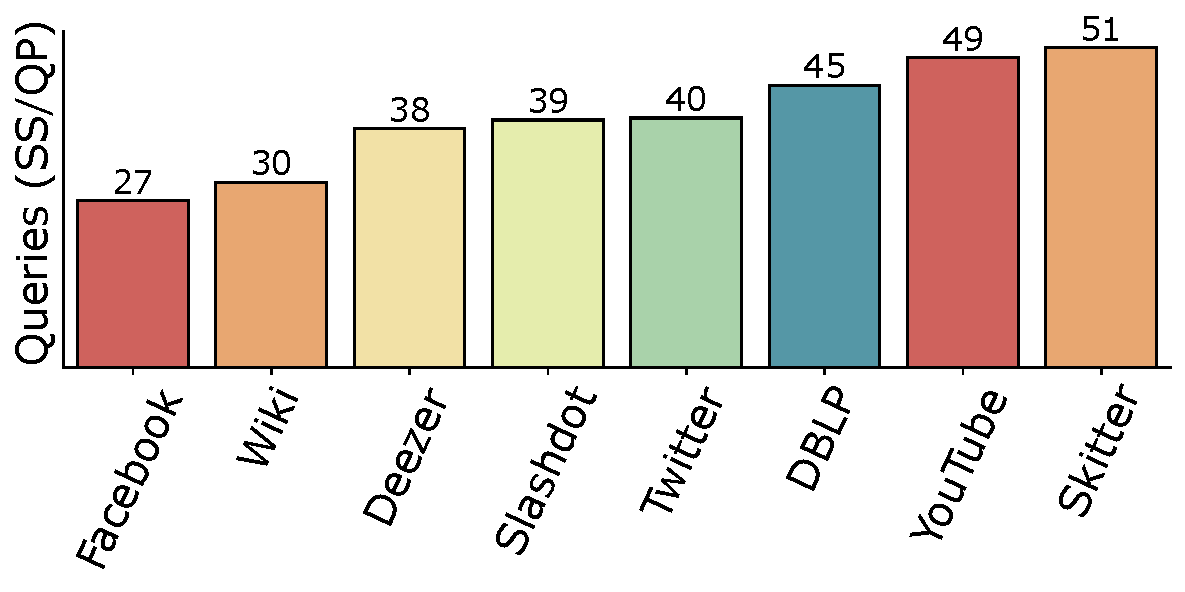
\includegraphics[width=0.5\textwidth]{Figures/Ratio/MaxCover_QueriesToPrune_inkspace.pdf}  
  \caption{ Comparison of the number of oracle calls between SS and \qs{}.}
  \label{fig:oracle_calls}

\end{figure}

In this section, we compare the empirical performance of \qs to
existing methods for the pruning problem across four different
objective functions, for both size and knapsack constraints.
The size constraint is the special case of the knapsack constraint
when $c(u) = 1$ for all $u \in \uni$ -- as the previous methods
for pruning are typically formulated for size constraint, this
allows for the fairest comparison with existing work. We provide the code and detailed instructions for reproducing the experiments in the supplementary material.

\textbf{Summary of results.} 
For both size and knapsack constraints,  we demonstrate
that \qs{} typically prunes over 90\% of the ground set
and sacrifices very little in terms of objective value,
achieving the highest combined metric (defined below) of
all pruning methods in
the majority of instances. 
The algorithm that is most competitive with \qs{} is
the Submodular Sparsification (SS) algorithm of  \citet{zhou2017scaling}.
However, SS requires $30$ times more oracle queries than \qs{}, as shown in Fig. \ref{fig:oracle_calls}.
For the ML-based pruning methods, a baseline \gnn that we introduce outperforms
the methods of
\gcomb{} \citep{manchanda2020gcomb}, \lense{} \citep{ireland2022lense}, and \comb{} \citep{tian2024combhelper}
on nearly every instance that we evaluated. 
Finally, in Section \ref{sec:multi_vs_single},
we show that  \qs{} improves over \qss{} by 5-10\% in objective value retained,
while increasing the size of the reduced ground set by less than 1\% percent. 

\textbf{Evaluation metrics.} We evaluate the algorithms using three performance metrics, where higher values indicate better performance in all cases. The first metric is the
\textit{pruning approximation ratio} $P_r$,
defined as the ratio of the objective value obtained from the pruned ground set $\uni'$ to the objective value from the original ground set $\uni$, both computed by a heuristic $\mathcal{H}$. Specifically, $P_r = f( \mathcal{H} (\uni')) / f( \mathcal{H} (\uni))$. The second metric is the
\textit{pruned fraction} $P_g$ of the original ground set that is pruned.
Finally, since an algorithm could trivially obtain the highest in one metric
by totally disregarding the other (pruning nothing or pruning everything),
we consider the \textit{combined metric}, $C = P_rP_g$.  

% $C = \log( P_r/ ( 1 - P_g ) )$ . 

In Appendix  \ref{appendix:heuristics},  we summarize the heuristics used for each application, noting that our heuristic-agnostic algorithm is flexible for use with any heuristic. We use only a single attempt to prune the ground set for all algorithms due to the computational cost.


 \textbf{Applications.} % \textcolor{blue}{Version 1:} We evaluate our algorithm on three classical CO problems on graphs: Maximum Cover (MaxCover), Maximum Cut (MaxCut), and Influence Maximization (IM). Additionally, we consider content-based information retrieval problem, where the goal is to find relevant content based on queries. For detailed specifications of these applications, see Appendix \ref{appendix:problem_formulation}.
We evaluate our algorithm on four applications: Maximum Cover (MaxCover), Maximum Cut (MaxCut), Influence Maximization (IM), and information retrieval. For detailed specifications of these applications, see Appendix \ref{appendix:problem_formulation}.




% \textcolor{blue}{Version 1 for Baselines:} 
\textbf{Baselines and Prior Methods.} We compare our algorithm against algorithms that accelerate heuristics by pruning the ground set rather than directly optimizing the objective function. Our evaluation include the following classical and learning based methods: Submodular Sparsification (SS) \citep{zhou2017scaling}, \gcomb{} \citep{manchanda2020gcomb}, \lense{} \citep{ireland2022lense}, \comb{} \citep{tian2024combhelper}, and \gnn{}, a proposed baseline, which is a modified version of \comb{}. While the authors of \comb{} stated that they used GCN \citep{kipf2016semi} as their choice of GNN, we observed that the implementation of the algorithm actually employs SAGEConv \citep{hamilton2017inductive}. To ensure a fair comparison, we have included both GNN options in our evaluation. Empirically, we find that replacing SAGECONV  in \comb{} with GCN  significantly improves the performance of \comb{}, as GCN retains information from all neighbors, unlike SAGECONV. Hence, our proposed baseline, \gnn, a modified version of \comb{}, uses a GCN with fewer layers and  uses random numbers as node features, eliminating the need for domain knowledge and extensive feature engineering. Moreover,  \gnn also outperforms the other ML methods, \lense{} and \gcomb{}.
% The authors of \comb{} mentioned using GCN \citep{kipf2016semi}, but the public implementation of \comb uses SAGEConv \citep{hamilton2017inductive}. 
 
For the general knapsack constraint, the prior methods do not easily generalize. Since \gnn{} does easily generalize and
outperformed the other ML-based methods on size constraints, we only compare to \gnn for general knapsack constraints.
Instead of using random numbers as node features, we provide the degree, cost, and degree-to-cost ratio of each node as input features
for \gnn. Additionally, we compare to the \topk{} approach, which selects a set (where the size of the set is equal to the size of the pruned ground set by \qs{}) consisting of the top $k$ degree-to-cost ratios. Further descriptions of each algorithm can be found in Appendix \ref{appendix:baselines}.




% \subsection{Datasets}
\textbf{Datasets.} We evaluate our approach using real-world datasets from the Stanford Large Network Dataset Collection \citep{leskovec2016snap} for the traditional CO problems on graph, following the experimental setup of \cite{ireland2022lense}. For experiments related to the
retrieval system, we use the Beans \citep{beansdata}, CIFAR100 \citep{Krizhevsky09learningmultiple},  FOOD101 \citep{bossard14} and UCF101 dataset \citep{soomro2012ucf101dataset101human}. A summary of all datasets used can be found in Appendix \ref{appendix:dataset}.




\begin{figure*}[ht] %{l}{0.6\textwidth}


  \subfigure{ %\label{fig:depend}
    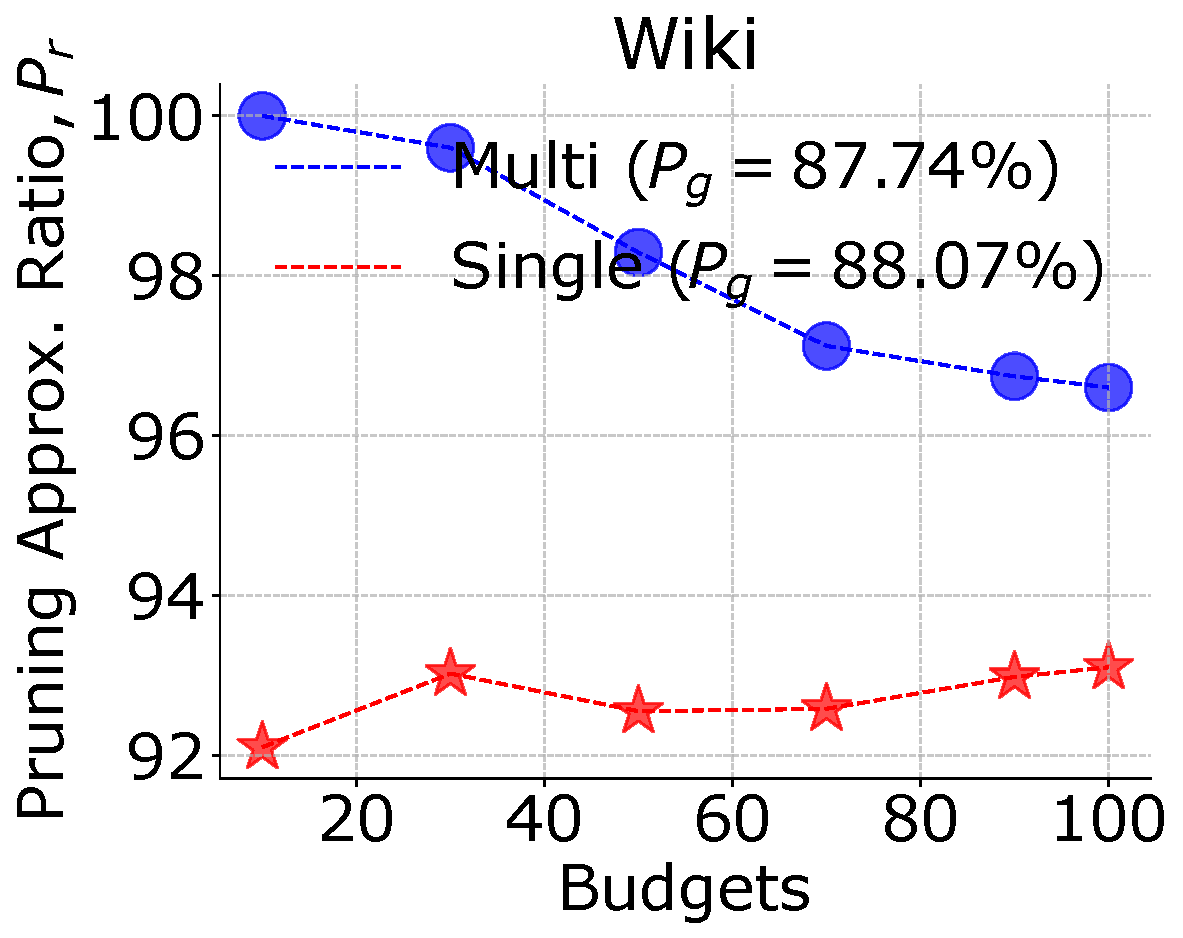
\includegraphics[width=0.23\textwidth]{Figures/IM/Wiki_inkspace.pdf}
  }
  \subfigure{ %\label{fig:depend}
    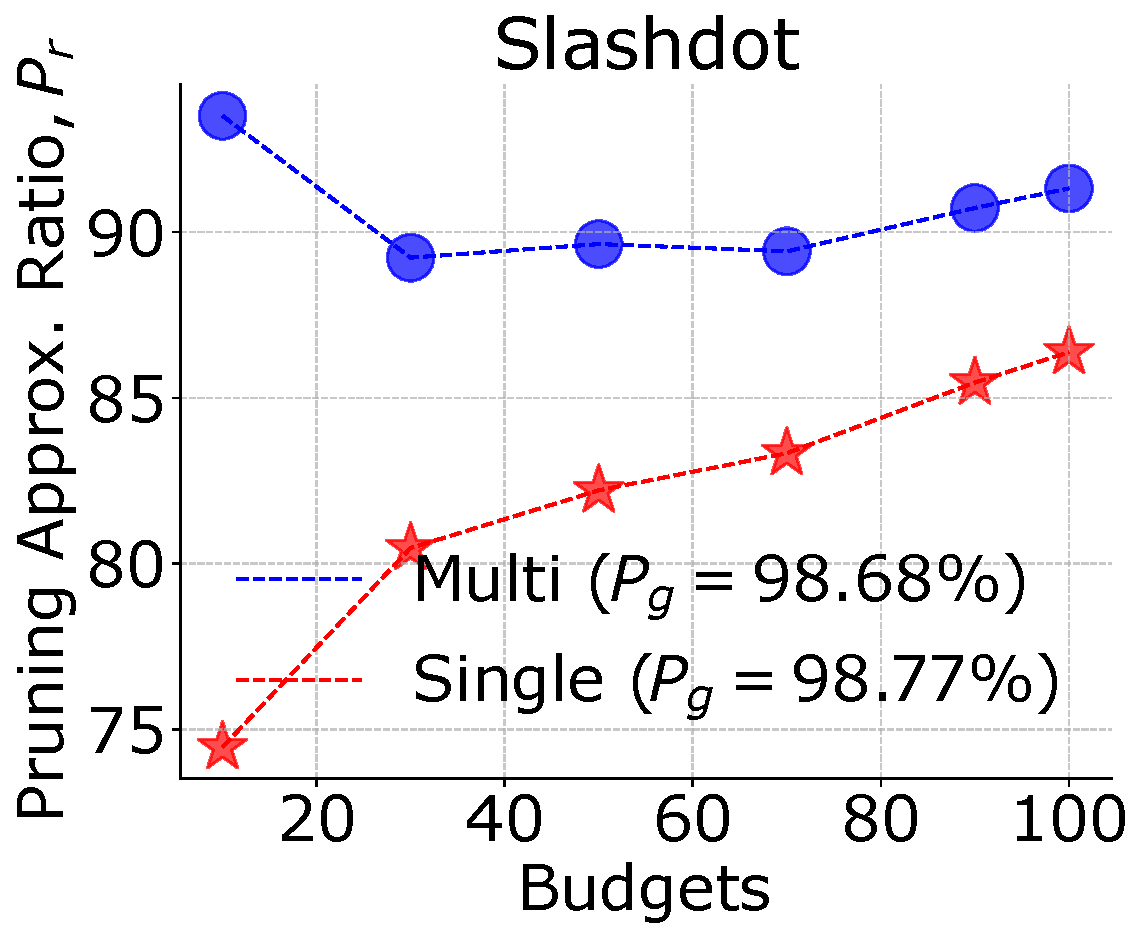
\includegraphics[width=0.23\textwidth]{Figures/IM/Slashdot_inkspace.pdf}
  }
  \subfigure{ %\label{fig:depend}
    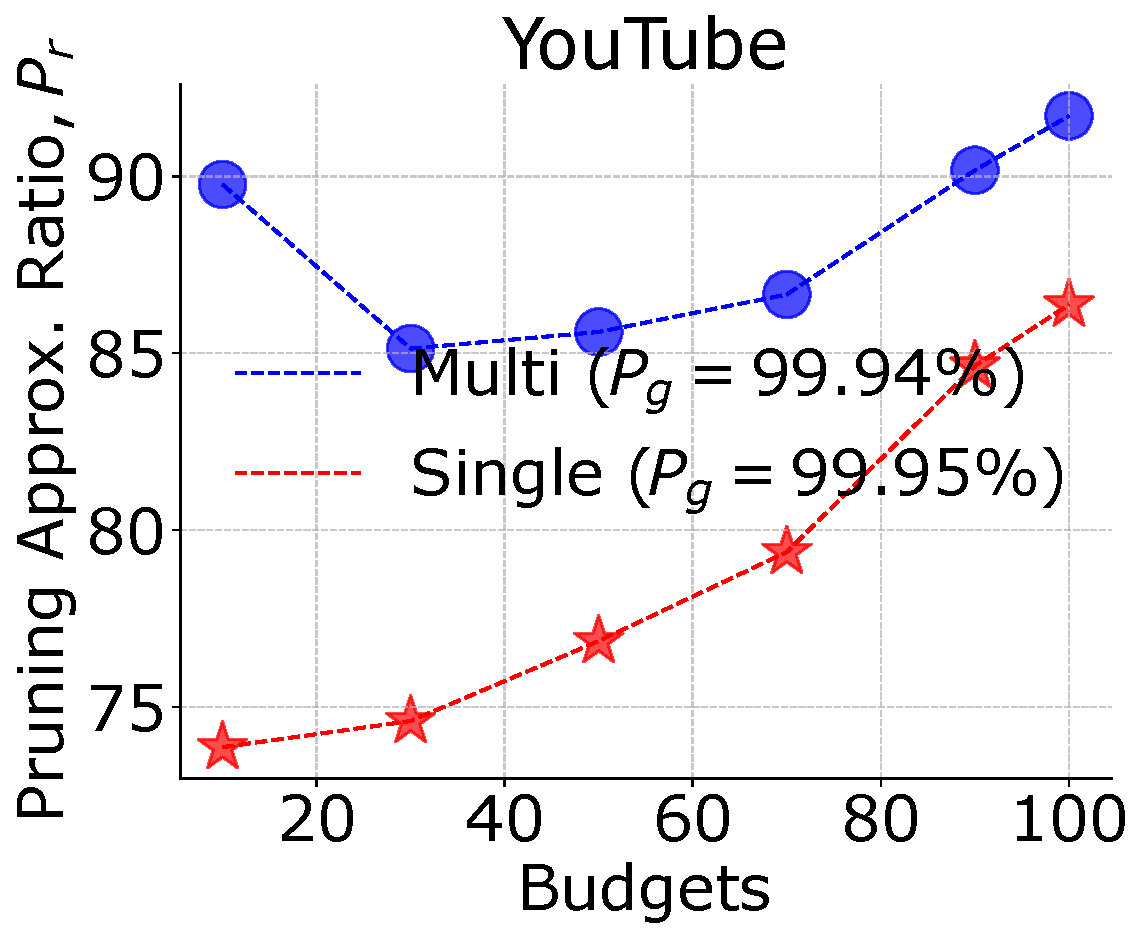
\includegraphics[width=0.23\textwidth]{Figures/IM/YouTube_inkspace.pdf}
  }
  \subfigure { %\label{fig:depend}
    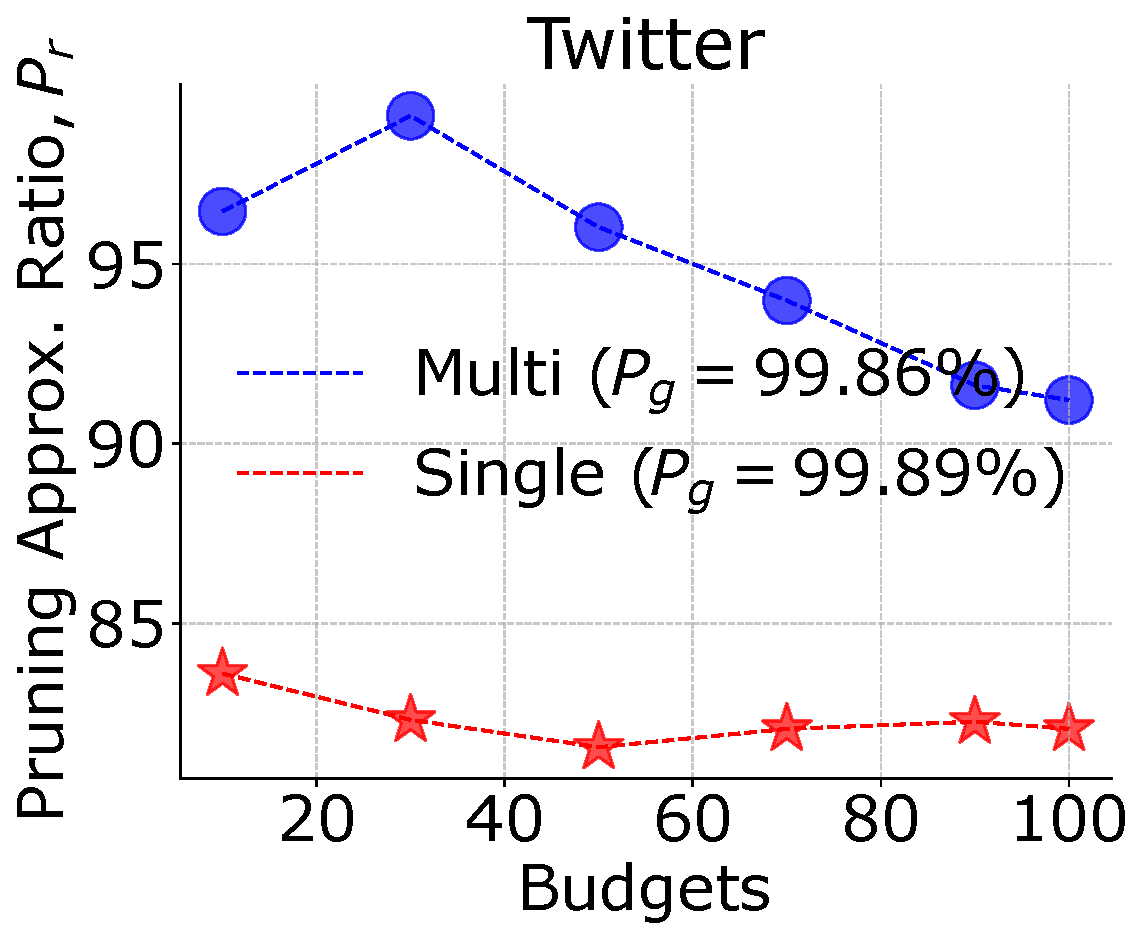
\includegraphics[width=0.23\textwidth]{Figures/IM/Twitter_inkspace.pdf}
  }
    
  \caption{Comparison between \qs and \qss  on a selection of data sets for IM.}
  \label{fig:main_paper_IM}
\end{figure*}


\subsection{Set 1: Evaluation on Size Constraints} \label{sec:size}
In this section, we evaluate the pruning methods for size constraints;
first for classical problems on graphs, and then for the image retrieval
application. 

\paragraph{Classical Problems on Graph.}
We consider traditional problems on graphs: Maximum Cover (MaxCover), Maximum Cut (MaxCut), and Influence Maximization (IM),
with a budget of $b=100$, following \cite{ireland2022lense}. From Table \ref{tab:size_constraint}, we observe that all algorithms achieve similar pruning approximation ratios. However, \qs{} is able to prune the original ground set by orders of magnitude more than most algorithms. Interestingly, and perhaps surprisingly, the IMM heuristic \citep{tang2015influence} occasionally achieves better solutions for IM
on the reduced ground set compared to the unpruned ground set (\eg Twitter, Wiki) -- which raises the intriguing
possibility of pruning to enhance the performance of a specific algorithm, which is out of the scope of this work. 

% We observe that for each problem and dataset, \qs{} is able to find an optimally pruned ground set while sacrificing little to no performance.
We observe that SS outperforms our method on some instances, particularly for IM.
However, as shown in Fig. \ref{fig:oracle_calls}, SS typically requires over $30$ times more oracle calls than \qs{}. Compared to other algorithms, \qs{} often surpasses these methods by orders of magnitude in pruning the ground set size while maintaining the same pruning approximation ratio. For example, \qs{} significantly outperforms \gcomb{} in pruning efficiency for MaxCover and MaxCut (we directly report the performance of \gcomb{} on these instances as reported in \cite{ireland2022lense}).

%We observe that machine learning algorithms may underperform due to their dependence on training data proportions and random splits between training and testing datasets, a phenomenon also reported in \citep{liang2024benchmark}.
We remark that, in contrast to our method, the learning-based approaches frequently require domain knowledge and extensive feature engineering. For instance, \lense{} uses eigenvector centrality as a node feature, which is a costly calculation for large graphs and necessitates extensive hyperparameter tuning for each dataset and problem. Similarly, \comb{} employs problem-specific boosting, requiring domain knowledge.
Nevertheless, even the best-performing machine learning approaches are less optimal than our method and require significantly higher computational overhead and running time. While LeNSE shows the lowest combined GPU and CPU memory usage among the ML approaches, \qs only utilizes CPU resources, which is less than the CPU usage of LeNSE alone. Please refer to Appendix \ref{appendix:scalability} for a detailed analysis of memory usage and runtime.
\paragraph{Image Retrieval System Results.}

Next, we present our results for the image retrieval system under size constraint. We randomly sampled five images from the query dataset and averaged the performance over ten such queries. Fig. \ref{fig:retrival_system}, provides an overview of the pipeline and results for the retrieval system. We compare our algorithm with SS and \random{} (which selects a random set of elements from the candidate dataset, with a size equal to that of \qs{}). Notice that on the CIFAR100 dataset, SS fails to complete pruning within the three-hour cut-off time. We observe that \qs{} outperforms \random{} but fails to outperform SS. Although SS performs better than our approach on the FOOD101 dataset, it returns a ground set that is $14$ times larger than ours.
% \vspace{-0.5em}
\subsection{Set 2: Performance on Knapsack Constraint}\label{sec:knapsack}
In this subsection, we compare our algorithm with the baselines for general knapsack constraints.

\textbf{Classical Problems on Graph.} We set the cost of each node following \cite{yaroslavtsev2020bring} (more details in Appendix \ref{appendix:problem_formulation}). In Table \ref{tab:knapsack_constraint}, we observe that \qs achieves the highest combined metric on 45\% of all instances tested. Specifically, for MaxCover and MaxCut, \qs often outperforms the simple baseline \topk{} by 20\% in retaining the objective value, except for Deezer-MaxCover and Skitter-MaxCut. The \topk{} approach does not account for the relationships between vertices, whereas \qs considers the problem more holistically, ensuring that the selected vertices collectively form a well-balanced subgraph. While \topk outperforms \qs for IM in most cases, its poor performance across MaxCut and MaxCover shows that \topk is not a robust approach across applications and datasets. On the other hand, \gnn performs quite well on some datasets but unexpectedly poorly on others.

% We set the cost of each node following \cite{yaroslavtsev2020bring} (more details in Appendix \ref{appendix:problem_formulation}).
% In Table \ref{tab:knapsack_constraint}, we present the  results for MaxCover and MaxCut.
% In summary, \qs achieves the highest combined metric on \textcolor{black}{56}\% of instances.
% We
% observe that \qs often outperforms the simple baseline \topk{} by 20\% in retaining the objective value, except for Deezer-MaxCover and Skitter-MaxCut. The \topk{} approach does not account for the relationships between the vertices, whereas \qs considers the problem more holistically, ensuring that the selected vertices collectively form a well-balanced subgraph. On the other hand, \gnn performs quite well on some datasets but unexpectedly poorly on others.
% % Although different architectures may alter the overall performance, we believe these experiments provide a reasonable understanding of the engineering effort required to improve machine learning approaches. 
% Additional results for the IM experiment are provided in Appendix \ref{appendix:qs_vs_baselines_IM}.
% \vspace{-1em}
\paragraph{Video Retrieval System Results.} We set the cost of each video proportional to its length.  For the video retrieval system, \gnn is not a suitable approach, as it cannot take a set of items as input. Therefore, we compare our approach with \random{} and \topk{} approach.
From Figure \ref{fig:video_summ}, we observe that \qs outperforms \random{} by 80\% while performing better than the \topk{} approach. 


% Please add the following required packages to your document preamble:
% \usepackage{multirow}
% \usepackage{graphicx}
% Please add the following required packages to your document preamble:
% \usepackage{multirow}
% \usepackage{graphicx}
% Please add the following required packages to your document preamble:
% \usepackage{multirow}
% \usepackage{graphicx}
% \begin{table*}[]
% \centering
% \caption{Comparison of pruning algorithms for knapsack constraint experiments (best in bold).\todo{add combined metric}}
% \vspace{1em}
% \label{tab:knapsack_constraint}
% \resizebox{\textwidth}{!}{%
% \begin{tabular}{lcccccccccccc}
% \hline
% \multirow{3}{*}{Graph}        & \multicolumn{6}{c}{Maximum Cover}                                                                                                                       & \multicolumn{6}{c}{Maximum Cut}                                                                                                                 \\ \cmidrule(lr){2-7} \cmidrule(lr){8-13}  
%                               & \multicolumn{2}{c}{\qs}                             & \multicolumn{2}{c}{\topk}                           & \multicolumn{2}{c}{\gnn}                    & \multicolumn{2}{c}{\qs}                             & \multicolumn{2}{c}{\topk}                           & \multicolumn{2}{c}{\gnn}            \\ \cline{2-13} 
%                               & $P_r \uparrow$ & $P_g$ $\uparrow$                 & $P_r \uparrow$ & $P_g$ $\uparrow$                 & $P_r \uparrow$ & $P_g$ $\uparrow$         & $P_r \uparrow$ & $P_g$ $\uparrow$                 & $P_r \uparrow$ & $P_g$ $\uparrow$                 & $P_r \uparrow$ & $P_g$ $\uparrow$ \\ \hline

% \multicolumn{1}{l|}{Facebook} & \textbf{97.25}& \multicolumn{1}{c|}{\textbf{98.71}} & 55.05& \multicolumn{1}{c|}{\textbf{98.71}
% } & 33.03          & \multicolumn{1}{c|}{99.36} & 98.99          & \multicolumn{1}{c|}{\textbf{96.66}} & \textbf{100.0} & \multicolumn{1}{c|}{\textbf{96.66}
% } & 96.67          & 49.84              \\
% \multicolumn{1}{l|}{Wiki}     & 94.00& \multicolumn{1}{c|}{\textbf{98.51}} & 75.50& \multicolumn{1}{c|}{\textbf{98.51}
% } & \textbf{100.0} & \multicolumn{1}{c|}{86.96} & 96.00          & \multicolumn{1}{c|}{\textbf{99.28}} & 51.00& \multicolumn{1}{c|}{\textbf{99.28}
% } & \textbf{100.0} & 18.36              \\
% \multicolumn{1}{l|}{Deezer}   & 87.50& \multicolumn{1}{c|}{\textbf{98.83}} & 91.50& \multicolumn{1}{c|}{\textbf{98.83}
% } & \textbf{100.0} & \multicolumn{1}{c|}{97.25} & 96.00          & \multicolumn{1}{c|}{\textbf{99.85}} & 80.00& \multicolumn{1}{c|}{\textbf{99.85}
% } & \textbf{100.0} & 97.45              \\
% \multicolumn{1}{l|}{Slashdot} & 89.50& \multicolumn{1}{c|}{\textbf{99.88}} & 57.00& \multicolumn{1}{c|}{\textbf{99.88}
% } & \textbf{100.0} & \multicolumn{1}{c|}{83.25} & 97.00          & \multicolumn{1}{c|}{\textbf{99.91}} & 67.00& \multicolumn{1}{c|}{\textbf{99.91}
% } & \textbf{100.0} & 43.95              \\
% \multicolumn{1}{l|}{Twitter}  & 87.00& \multicolumn{1}{c|}{\textbf{99.87}} & 59.50& \multicolumn{1}{c|}{\textbf{99.87}
% } & \textbf{100.0} & \multicolumn{1}{c|}{43.83} & 95.00          & \multicolumn{1}{c|}{\textbf{99.96}} & 29.00& \multicolumn{1}{c|}{\textbf{99.96}
% } & \textbf{100.0} & 2.25               \\
% \multicolumn{1}{l|}{DBLP}     & 84.50& \multicolumn{1}{c|}{\textbf{99.97}} & 71.50& \multicolumn{1}{c|}{\textbf{99.97}
% } & \textbf{100.0} & \multicolumn{1}{c|}{99.71} & 95.00          & \multicolumn{1}{c|}{\textbf{99.99}} & 43.00& \multicolumn{1}{c|}{\textbf{99.99}
% } & \textbf{100.0} & 99.88              \\
% \multicolumn{1}{l|}{YouTube}  & 91.50& \multicolumn{1}{c|}{\textbf{99.99}} & 52.00& \multicolumn{1}{c|}{\textbf{99.99}
% } & \textbf{100.0} & \multicolumn{1}{c|}{36.26} & 97.00          & \multicolumn{1}{c|}{\textbf{99.99}} & 73.00& \multicolumn{1}{c|}{\textbf{99.99}
% } & \textbf{100.0} & 94.06              \\
% \multicolumn{1}{l|}{Skitter}  & 90.50& \multicolumn{1}{c|}{\textbf{99.99}} & 81.50& \multicolumn{1}{c|}{\textbf{99.99}} & \textbf{100.0} & \multicolumn{1}{c|}{98.87} & 97.00          & \multicolumn{1}{c|}{\textbf{99.99}} & \textbf{100.0} & \multicolumn{1}{c|}{\textbf{99.99}} & \textbf{100.0} & 99.93              \\ \hline

% \end{tabular}%
% }
% \end{table*}
\subsection{Set 3: Multi-Budget and  Single-Budget Comparison} \label{sec:multi_vs_single}

Finally, we compare the performance of \qs and \qss (which prunes for the maximum budget) for a range of budget.
Following the multi-budget analysis in \cite{ireland2022lense}, we vary the budget $b$ from $10$ to $100$.
We remark that for size constraint, no significant improvement is observed for  \qs{} over \qss{} in the size-constrained experiments
-- we speculate that this may be at least partially explained by the efficacy of the standard greedy
algorithm for the size constraint, and a greedy solution of smaller size is automatically
contained in greedy solutions of larger sizes. 
However, for general knapsack constraint,
we observe that \qs  typically improves by 3\%-10\% over \qss{} for IM (Figure \ref{fig:main_paper_IM}), 
while only increasing the size of the ground set less than 1\% percent. \textcolor{black}{For MaxCover, we observe qualitatively similar
  improvements on some datasets; however, for MaxCut, \qs and \qss perform similarly.}
We provide results for each application and dataset in Appendix \ref{appendix:multi_vs_single}.












%%% Local Variables:
%%% mode: latex
%%% TeX-master: "main.tex"
%%% End:
